\documentclass[twocolumn,11pt,uplatex]{jsarticle}
\usepackage[dvipdfmx]{graphicx}
\usepackage[top=15truemm,bottom=15truemm,left=20truemm,right=20truemm]{geometry}
\usepackage{setspace}
%\usepackage{}
\setlength{\columnsep}{3zw}

\begin{document}
 \twocolumn
 [
  \begin{center}
   {\normalsize \textrm{平成27年度 修士論文要旨}}
   \\
   \vspace{0.15cm}
   {\Large \textrm{陽子--$^3$He散乱実験に向けた\\RbのESR測定による$^3$He偏極度測定システムの開発}}
   \\
   \vspace{0.15cm}
   {\large \textrm{東北大学理学研究科 物理学専攻 原子核物理研究室}}
   \\
   {\large \textrm{渡邉 跡武}}
   \vspace{0.2cm}
  \end{center}
 ]
 
 \setstretch{0.87}
 \pagestyle{empty}
 
\section{研究背景}
核力の理論的記述は、1935年に提唱された湯川秀樹の中間子理論に始まり、1990年代には二核子間での核力を記述する現実的な二体核力ポテンシャルが完成した。\\\
 一方で、三つの核子間で同時に相互作用が起こる三体核力の存在も示唆されていた。現に、$^3$Hや$^3$Heといった核子数が3の原子核の束縛エネルギーは二体核力のみでは再現できず、三体核力を考慮することで不一致が解消されている。\\
 我々は、核子数が4の散乱系における三体核力の性質を詳細に調べていくために、陽子--$^3$He弾性散乱の完全測定を目標としている。そのためには微分断面積だけでなく$^3$He偏極分解能$A_y$等のスピン観測量の測定も必要である。陽子--$^3$He弾性散乱によって$A_y$を測定するためには偏極$^3$He標的が不可欠である。我々は$A_y$を統計誤差$\delta A_y \le 0.02$で測定するために$25$%以上の偏極度をもつ偏極$^3$He標的の開発を行ってきた\cite{wada, shiokawa}。先行研究では約$5$%の$^3$He偏極度が得られており、偏極度の更なる向上が求められる。また$^3$He偏極度の絶対値を高精度で測定するシステムの確立も要請される。


\section{本研究の目的}
現在我々が$^3$He偏極度の測定方法として採用している高速断熱通過-核磁気共鳴(AFP-NMR)法では、検出回路系の$Q$値等が不確定なためにNMR信号強度から偏極度の絶対値へ較正する時の誤差が大きい。\\
 $^3$He原子核を偏極させる方法としては、スピン交換光ポンピング法を採用している。これは円偏光レーザーによって静磁場中のRb原子を偏極させ、Rb原子と$^3$He原子核とのスピン交換反応によって$^3$He原子核を偏極させる方法である。この時、混合気体中のRbの電子スピン共鳴(ESR)周波数が、偏極した$^3$He原子核によってシフトすることが知られており、その周波数シフトを測定することで$^3$He偏極度を求めることが出来る。\\
 本研究の目的は、$^3$He偏極度の絶対値を高精度で測定し、AFP-NMR法の較正を行うために、RbのESR周波数シフト測定による新たな$^3$He偏極度測定システムを開発することである。また開発する測定システムにおける$^3$He偏極度の測定精度は$10$%以下を目標とした。


\section{$^3$He偏極度測定システムの開発}
RbのESR周波数シフトは、$^3$Heの核スピンの向きを反転させ、静磁場に対して平行または反平行それぞれの状態でのESR周波数を測定し、それらの差をとることで求められる。$^3$HeガスおよびRbが封入されたガラスセルに振動磁場をかけ、光ポンピングによって励起されたRbの遷移を誘起し、その時放出される蛍光強度が最大となる振動磁場の周波数がESR周波数となる。本研究で開発したRbのESR周波数シフト測定システムの概略図を図\ref{ESR_setup}に示す。
%
 \begin{figure}[htbp]
  \centering
   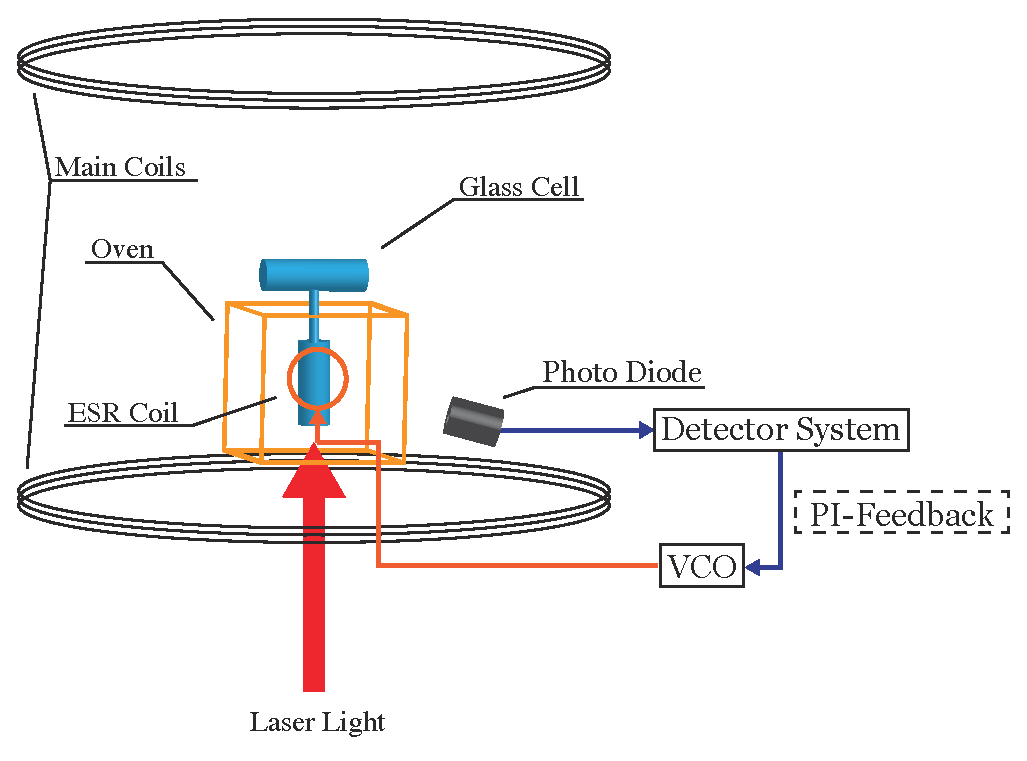
\includegraphics[width=7.5cm]{ESR_setup_abst.pdf}
   \caption{ESR周波数シフト測定システムの概略図}
   \label{ESR_setup}
 \end{figure}
%
静磁場はメインコイルによって作られ、また円偏光レーザーはガラスセルの下部から照射される。ガラスセルはダブルセル構造であり、Rbを含んだポンピング部をオーブンに入れ加熱することでRb蒸気を発生させた。また振動磁場を印加するためのESRコイルをオーブン内に入れ、外部入力によって周波数を変調できる電圧制御発振器(VCO)に接続した。ESR周波数は静磁場の大きさに依存するので、静磁場の揺らぎによってESR周波数も変化してしまう。そこで、フォトダイオードによって観測した蛍光強度を利用したフィードバック回路を組み込むことで、常に振動磁場の周波数が共鳴周波数付近に変調されるようにした。RbのESR周波数シフトの測定結果を図\ref{ESRshift}に示す。測定結果から、$^3$Heの核スピンの向きによるESR周波数シフトを確認することに成功した。

 \begin{figure}[tbp]
  \centering
   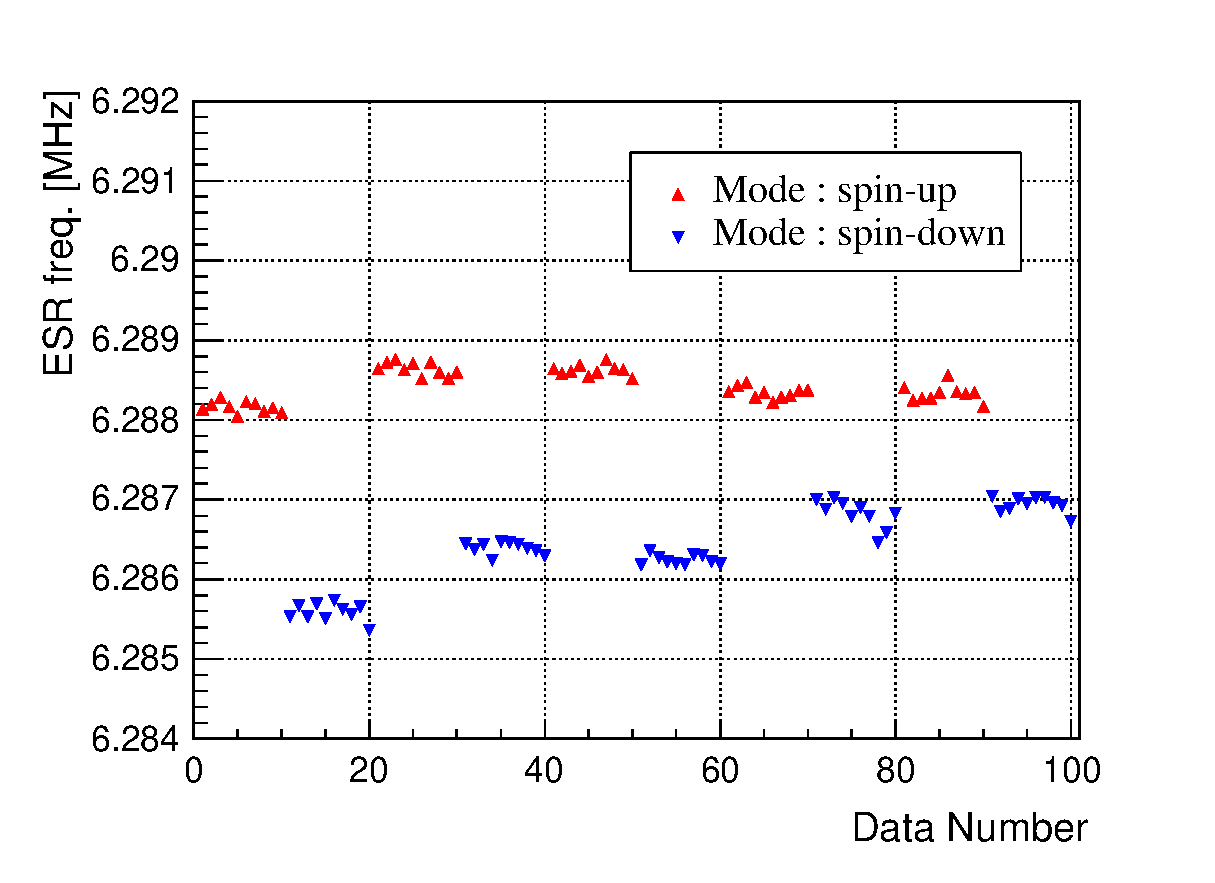
\includegraphics[width=7.5cm]{ESRfreq_ave_abst.eps}
   \caption{ESR周波数シフトの測定結果}
   \label{ESRshift}
 \end{figure}

AFP-NMR法の較正は、$^3$Heの核スピンをAFP法によって反転させる時にNMR測定も同時に行い、それによって得られたNMR信号強度と、RbのESR周波数シフト測定によって得られた$^3$He偏極度を対応させることで行った。これらの測定によって得られたNMR信号強度$V_{\rm NMR}$に対するESR周波数シフト$\Delta \nu_{\rm ESR}$の関係図を図\ref{ESRshift-Vnmr}に示す。また図\ref{ESRshift-Vnmr}にはESR周波数シフトから計算した$^3$He偏極度$P_{\rm ^3He}$も右側の縦軸に示している。

 \begin{figure}[htbp]
  \centering
   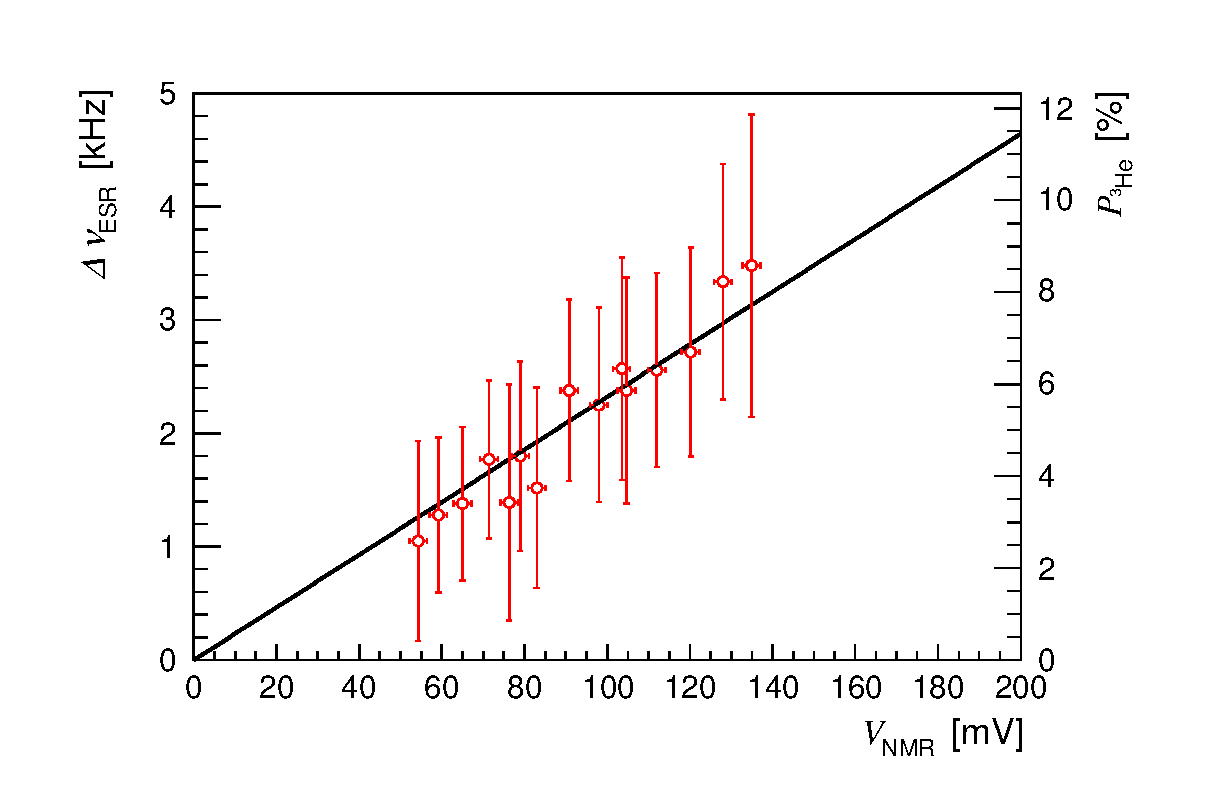
\includegraphics[width=7.5cm]{ESRfreq-Vnmr_abst.eps}
   \caption{NMR信号強度とESR周波数シフトおよび$^3$He偏極度との関係図}
   \label{ESRshift-Vnmr}
 \end{figure}

図\ref{ESRshift-Vnmr}の実線は、原点を通る一次関数でフィッティングした結果である。フィッティングの結果から、NMR信号強度と$^3$He偏極度の関係式は
%
\begin{equation}
 P_{\rm ^3He}~[%] = (5.72 \pm 0.61) \times 10^{-2} V_{\rm NMR}~[{\rm mV}]
 \label{Vnmr-P_3He}
\end{equation}
%
となり、$^3$He偏極度の測定精度は約$11$%となった。この時、その他の系統誤差は$1$%以下であった。


\section{陽子--$^3$He弾性散乱実験による$^3$He偏極分解能測定}
$^3$He偏極分解能$A_y$を求めるために、東北大学CYRICにおいて$70~{\rm MeV}$の陽子ビームを用いた陽子--$^3$He弾性散乱実験を行った。実験中は定期的にNMR測定を行った。実験中のNMR信号強度から、$^3$He偏極度は$10〜11$%程度であった。\\
 $A_y$の測定は、実験室系の角度$55^{\circ}$および$70^{\circ}$に設置された検出器によって散乱陽子を検出することで行った。AFP-NMR法によって$^3$Heの核スピンを反転させ、その前後における散乱陽子数の非対称度から$A_y$と$^3$He偏極度の積が求められる。式(\ref{Vnmr-P_3He})を用いて実験中の$^3$He偏極度を求め、その値から
%
\begin{eqnarray}
 A_y(55^{\circ}) &=& -0.35 \pm (0.01)_{\rm stat} \\
 A_y(70^{\circ}) &=& -0.33 \pm (0.03)_{\rm stat}
\end{eqnarray}
%
を得た。ここで、$A_y$の誤差としては統計誤差のみを示している。一方で、$A_y$の系統誤差は前述した$^3$He偏極度の測定精度によるものに加えて、散乱測定系の系統誤差が含まれる。散乱測定系の系統誤差を評価するために、非偏極の$^3$He標的を用いた擬非対称度の測定を行った。測定の結果、式(2,3)における$A_y$に対して$30$%程度の散乱測定系の系統誤差が得られた。

\section{まとめと展望}
$^3$He偏極度の絶対値を測定するために、RbのESR周波数シフト測定による$^3$He偏極度測定システムの開発を行った。開発したシステムによって測定を行い、ESR周波数シフトを確認した。また、その値から$^3$He偏極度を求め、AFP-NMR法の較正を行った。$^3$He偏極度の測定精度は、約$11$%の値を達成した。\\
 東北大学CYRICで陽子--$^3$He弾性散乱実験による$A_y$の測定を行った。$A_y$の誤差としては$^3$He偏極度の測定精度および散乱測定系の系統誤差が支配的であることが分かった。散乱測定系の系統誤差は、$^3$He偏極度を向上させることで相対的に小さくすることが出来る。\\
 今後はより高精度で$A_y$を測定するために、$^3$He偏極度の更なる向上を図ると共に、本研究で開発したRbのESR周波数シフト測定システムの測定精度の向上も行っていく予定である。
 
\begin{thebibliography}{99}

% \bibitem{WJS95}
% R. B. Wiringa, V. G. J. Stoks, and R. Schiavilla, Phys. Rev. C $\bf 51$, 38 (1995).
% \bibitem{Mac01}
% R. Machleidt, Phys. Rev. C $\bf 63$, 024001 (2001).
% \bibitem{Sto94}
% V. G. J. Stoks $\it et \ al.$, Phys. Rev. C $\bf 49$, 2950 (1994).
% \bibitem{Sek02}
% K. Sekiguchi $\it et~al$, Phys. Rev. C $\bf 65$, 034002 (2002).
% \bibitem{Sek11}
% K. Sekiguchi $\it et~al$, Phys. Rev. C $\bf 83$, 061001 (2011).
 \bibitem{wada}
 和田泰敬, 修士論文, 東北大学 (2013).
 \bibitem{shiokawa}
 塩川裕太, 修士論文, 東北大学 (2014).
 
\end{thebibliography}

\end{document}